\section*{Main equations:}

\vspace{-5 mm}

\begin{table}[H]
    \centering
    \scalebox{1.3}{
    \begin{tabular}{|lr|}\hline 
     \rowcolor{yellow}{
    {\bf Motion:}&}
    \\\hline
    \rowcolor{gray!50}{
    {\bf Studied motions:} One dimensional motions. Straight line motion.}
    &\\\hline
    \rowcolor{white}{
    {\bf UM: Uniform Motion (constant velocity)}}
    &\\
    \rowcolor{white}{
    {\bf UAM: Uniformly Accelerated Motion (constant acceleration)}}
    &\\\hline
    \rowcolor{gray!50}{
    {\bf Variable definition:}}
    &\\\hline
    {\bf Distance,} $\bm{d:}$ Quantity of space between two points along a path.&\\
    {\bf Displacement,} $\bm{\vec{d}:}$ Relative distance and direction between two positions. &\\
    {\bf Average speed,} $\bm{v:}$ Increment of the distance per time unit. &\\
    {\bf Average velocity,} $\bm{\vec{v}:}$ Increment of the displacement per time unit. &\\
    {\bf Rate of change of speed,} $\bm{a:}$ Increment of the average speed per time unit. &\\
    {\bf Average acceleration,} $\bm{a:}$ Increment of the average velocity per time unit. &\\\hline
    %
    %
    %
    %
    %
    \rowcolor{yellow}{
    {\bf SCALAR VARIABLES: Average speed $\bm v$ relations:}}
    &\\\hline
     \rowcolor{blue!20}{\bf Average speed - distance - time} \textcolor{red}{\bf It can be used always}    &  \\
     %
     \vspace{-1.5 mm}
     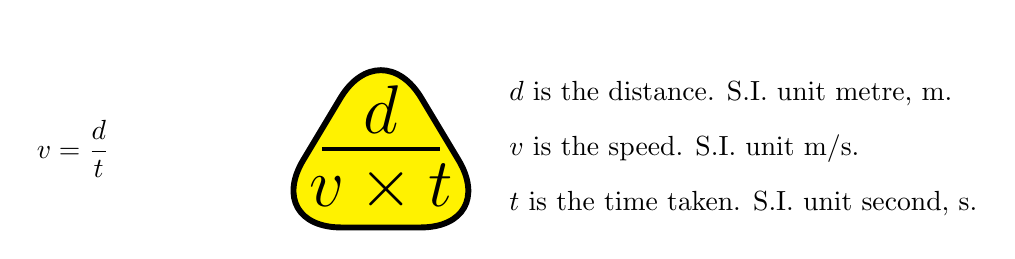
\begin{tikzpicture}[thick,scale=1.0, every node/.style={transform shape}]
    \draw[rounded corners=10mm,draw=black,line width = 0.75mm,fill=yellow] (0,0) -- (3,0) -- (1.5,2.5) --cycle;
    \draw[line width = 0.5mm] (0.75,1) -- (2.25,1);
    \node[at={(1.5,0.5)},color=black]{\Huge $v\times t$};
    \node[at={(1.5,1.5)},color=black]{\Huge $d$};
    \node[right] at (3,1.7) {$\bm{d}$ is the distance. S.I. unit metre, m.};
    \node[right] at (3,1) {$\bm v$ is the speed. S.I. unit m/s.};
    \node[right] at (3,0.3) {$\bm{t}$ is the time taken. S.I. unit second, s.};
    \node[right] at (-3,1) {$\displaystyle{\bm{v=\frac{d}{t}}}$};
    \end{tikzpicture} &
     %
     \\
     \rowcolor{red!20}{\bf Average speed - initial speed - final speed:}  & \\
     $\displaystyle{\bm{v=\frac{v_\text{i}+v_\text{f}}{2}}}$ \hspace{1cm} Can be used \textcolor{red}{only} for UM or UAM & \\
     \rowcolor{gray!20}{\bf Rate of change of speed - initial and final speed - time:}    &  \\
     $\displaystyle{\bm{ a=\frac{v_\text{f}-v_\text{i}}{t}}}$ \hspace{1cm} It is just the module of acceleration. Always valid. & \\\hline
     \rowcolor{yellow}{
    {\bf VECTORIAL VARIABLES: Average velocity $\bm{\vec{v}}$ relations:}}
    &\\\hline
     \rowcolor{blue!20}{\bf Average velocity - displacement - time: \textcolor{red}{\bf It can be used always}}    &  \\
     %
     %
     %
      %
     \vspace{-1.5 mm}
     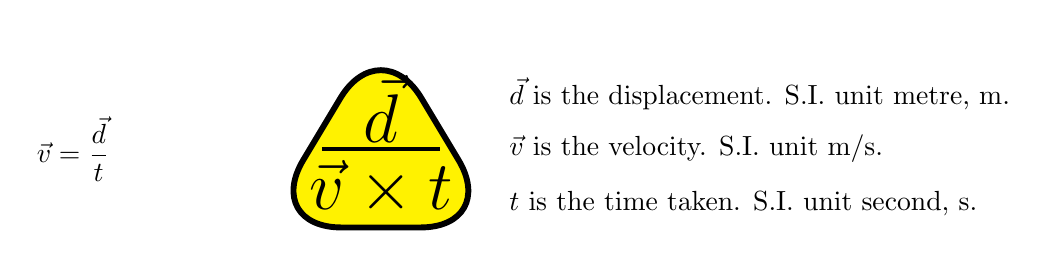
\begin{tikzpicture}[thick,scale=1.0, every node/.style={transform shape}]
    \draw[rounded corners=10mm,draw=black,line width = 0.75mm,fill=yellow] (0,0) -- (3,0) -- (1.5,2.5) --cycle;
    \draw[line width = 0.5mm] (0.75,1) -- (2.25,1);
    \node[at={(1.5,0.5)},color=black]{\Huge $\vec{v}\times t$};
    \node[at={(1.5,1.5)},color=black]{\Huge $\vec{d}$};
    \node[right] at (3,1.7) {$\bm{\vec{d}}$ is the displacement. S.I. unit metre, m.};
    \node[right] at (3,1) {$\bm{\vec{v}}$ is the velocity. S.I. unit m/s.};
    \node[right] at (3,0.3) {$\bm{t}$ is the time taken. S.I. unit second, s.};
    \node[right] at (-3,1) {$\displaystyle{\bm{\vec{v}=\frac{\vec{d}}{t}}}$};
    \end{tikzpicture} &\\
     \rowcolor{red!20}{\bf Average velocity - initial velocity - final velocity:}    &  \\
     $\displaystyle{\bm{\vec{v}=\frac{\vec{v}_\text{i}+\vec{v}_\text{f}}{2}}}$ \hspace{1cm} Can be used \textcolor{red}{only} for UM or UAM & \\
     {\rowcolor{gray!20}\bf Average acceleration - initial and final velocity - time:}    &  \\
     $\displaystyle{\bm{ \vec{a}=\frac{\vec{v}_\text{f}-\vec{v}_\text{i}}{t}}}$ \hspace{1cm} Can be used always & \\\hline
    \end{tabular}}
\end{table}

%
\newpage

\begin{figure}[H]
    \centering
    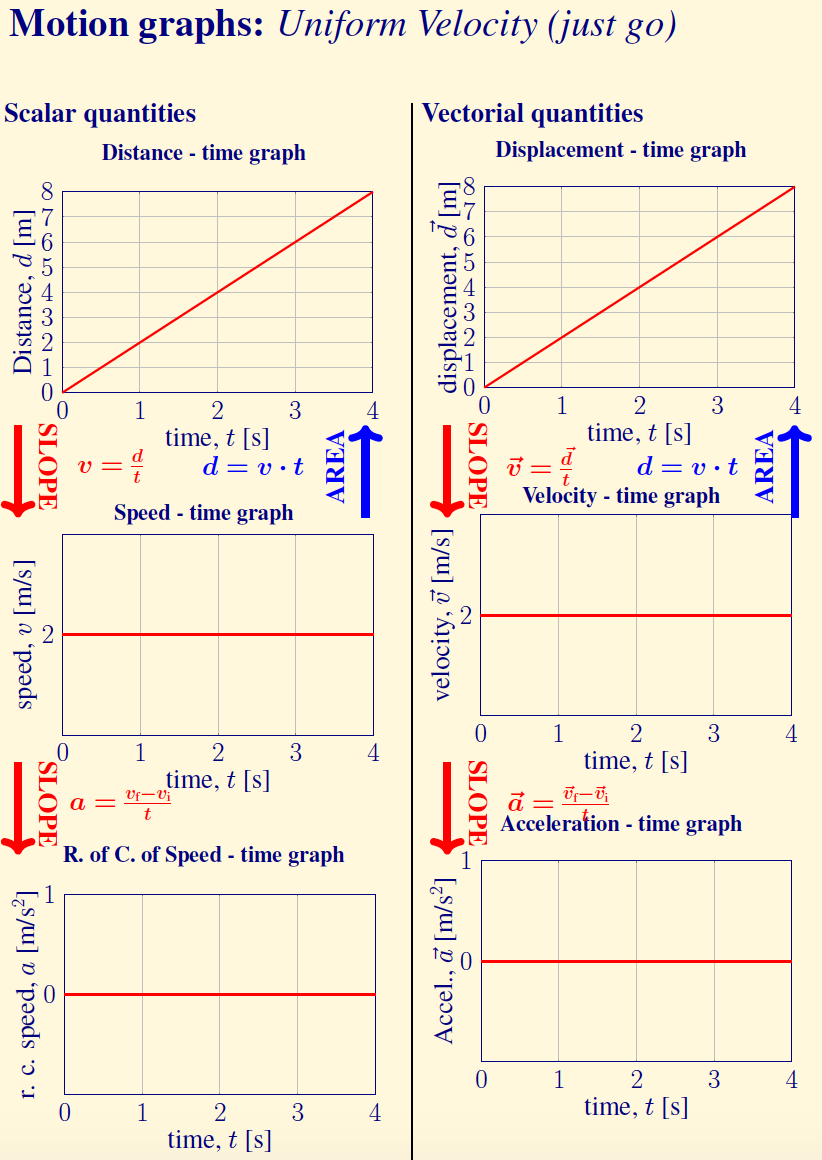
\includegraphics[scale=1.1]{FIG1.png}
\end{figure}

\newpage

\begin{figure}[H]
    \centering
    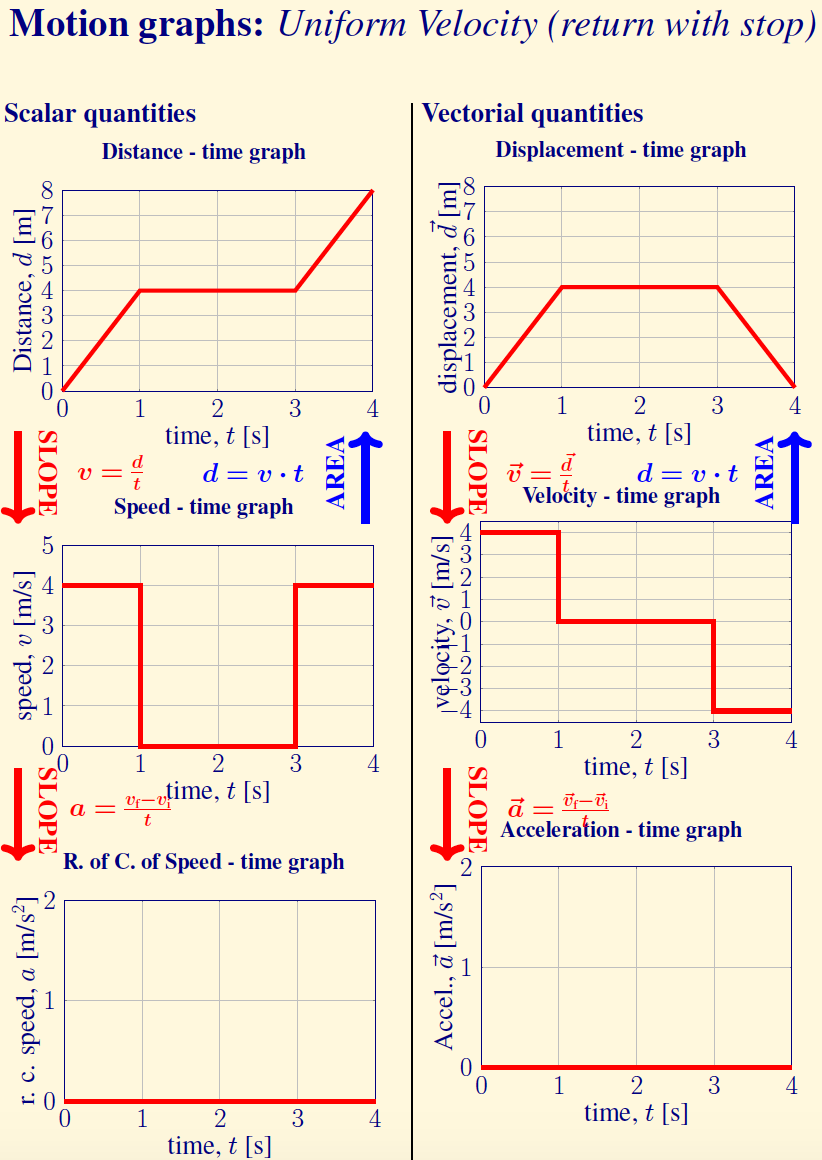
\includegraphics[scale=1.1]{FIG2.png}
\end{figure}

\newpage

\begin{figure}[H]
    \centering
    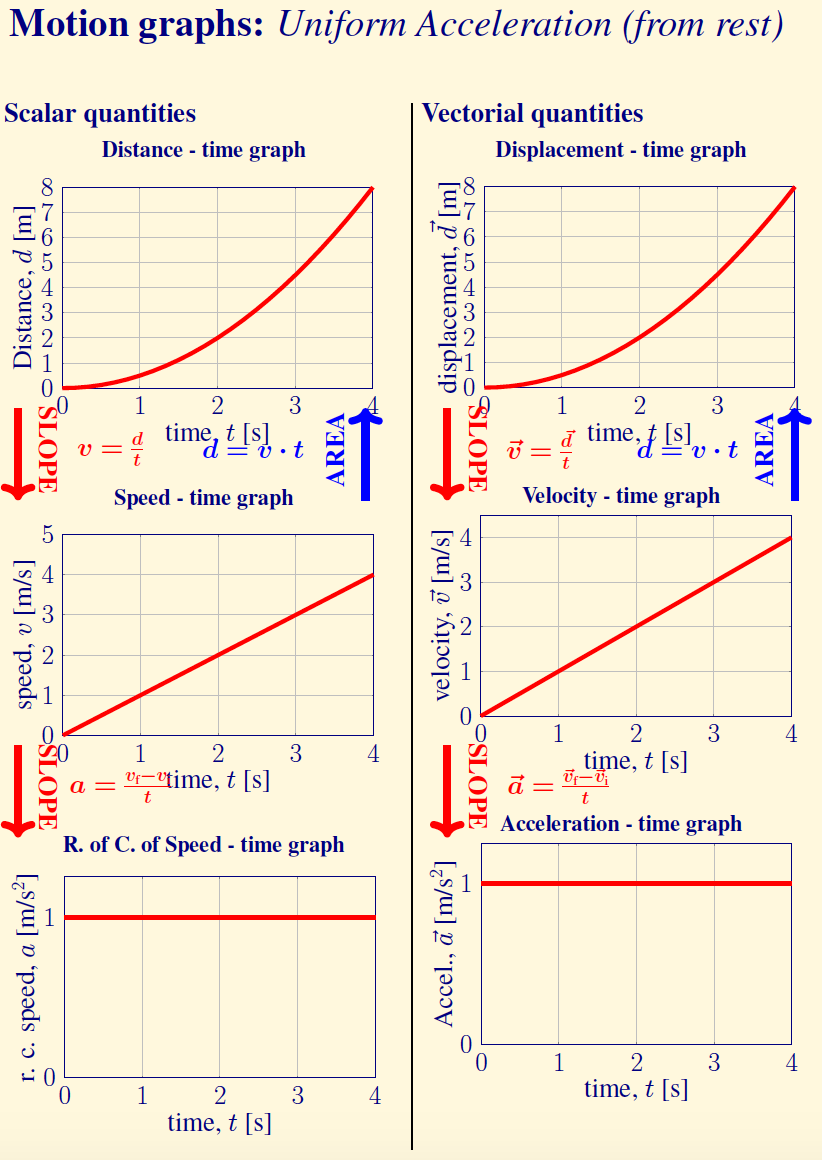
\includegraphics[scale=1.1]{FIG3.png}
\end{figure}

\newpage

\begin{figure}[H]
    \centering
    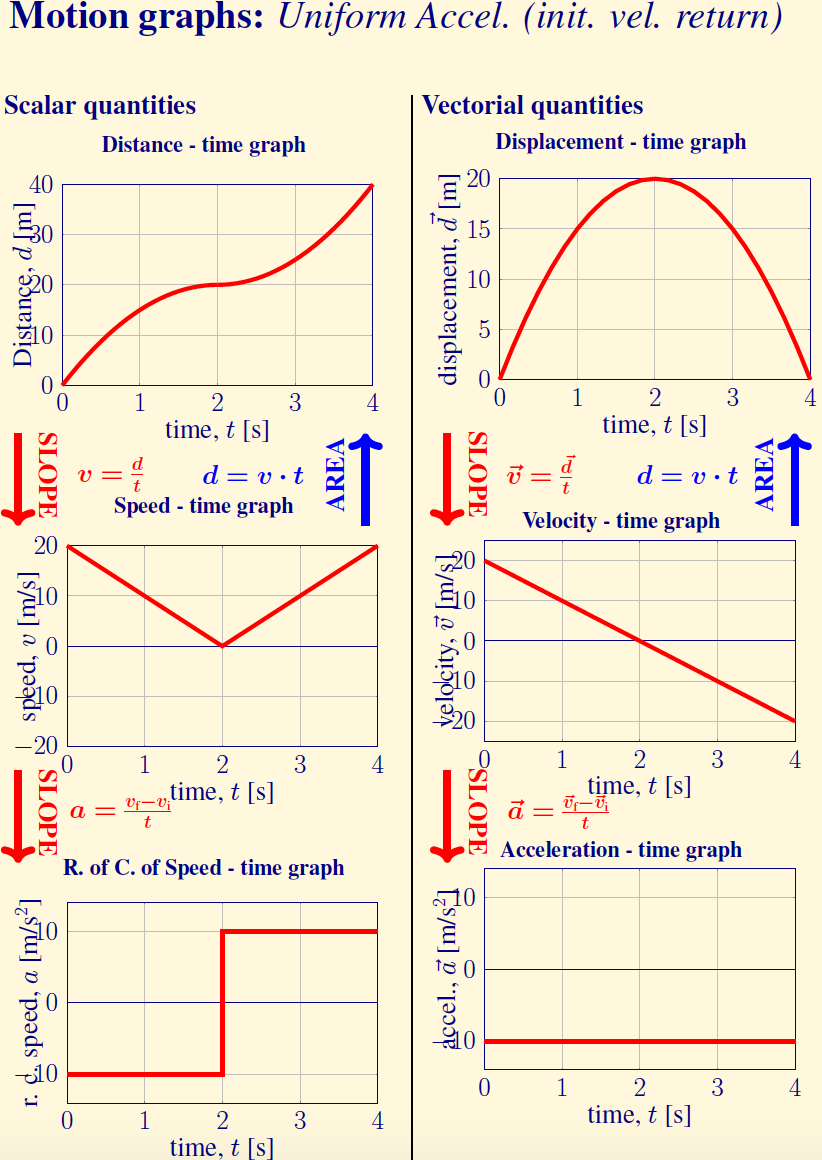
\includegraphics[scale=1.1]{FIG4.png}
\end{figure}

\newpage